%!TEX ROOT=../diploma-thesis.tex

\chapter{Návrh frameworku}\label{ch:navrh}

V této kapitole je diskutován návrh frameworku pro centrální správu
a automatickou integraci business pravidel vyhovující požadavkům identifikovaným
v sekci~\ref{sec:implementation-requirements}. Tento návrh staví na znalostech získaných
v předchozí kapitole~\ref{ch:reserse}, zejména na paradigmatu \gls{AOP} a přístupu \gls{ADDA}.

\section{Formalizace architektury orientované na služby}

Pro formalizaci problému byznysových pravidel v \gls{SOA} do termínů \gls{AOP} je nutno
identifikovat \textit{join-points}, určit podobu \textit{advices}, popsat způsob jakým budou
zachyceny \textit{pointcuts} a nakonec navrhnout proces \textit{weavingu} pravidel.

\subsection{Join-points}

Identifikace join-points vychází ze životního cyklu služby, který je znázorněn
na obrázku~\ref{fig:join-points}. První fází v životě instance služby je její inicializace,
konkrétně načtení aplikačního kontextu. V tomto bodě je potřeba získat veškerá pravidla, která
bude služba potřebovat ke své funkci.
Po inicializaci vstupuje služba do fáze, ve které může přijímat požadavky
na vykonání byznysových operací. Při přijmutí požadavku je nejprve nutno určit
byznysový kontext a poté vyhodnotit veškeré \textit{preconditions}. Pokud jsou všechny předpoklady
pro spuštění operace splněny, může být vykonána. Po dokončení operace je nutno aplikovat relevantní
post-conditions.

\begin{figure}
    \centering
    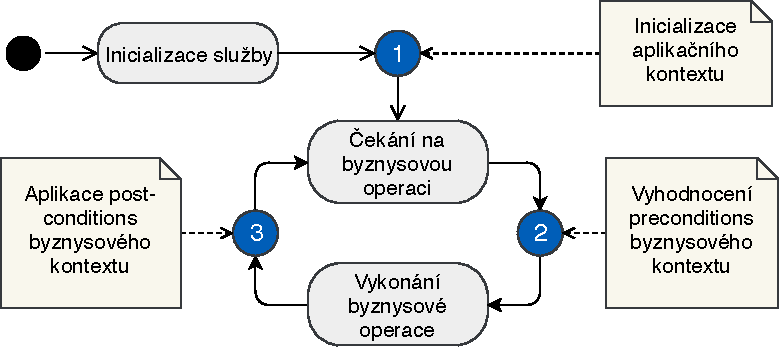
\includegraphics[keepaspectratio=true, width=0.6\linewidth]{figures/join-points.pdf}
    \caption{Diagram životn\'{\i}ho cyklu služby a identifikovan\'ych join-pointů}
    \label{fig:join-points}
\end{figure}

Identifikované join-points tedy jsou:

\benum[label=\circledarabic]
\item\label{itm:initialization} Inicializace instance služby
\item\label{itm:before} Volání byznysové operace
\item\label{itm:after} Dokončení byznysové operace
\eenum

\subsection{Pointcuts}

V join-pointu~\ref{itm:initialization} by služba měla načíst všechna byznysová pravidla, která
bude potřebovat ke své činnosti, a nejsou pro ni lokálně dostupná. Služba tedy musí zjistit,
která pravidla je potřeba získat, a následně si je vyžádat od ostatních služeb.
V join-pointech~\ref{itm:before}~a~\ref{itm:after} musejí být aplikována byznysová pravidla každého
kontextu vztahujícího se k dané operaci.

\lstinputlisting[
caption={Ukázka zápisu validačních pravidel pomocí anotací v jazyku Java},
label={lst:jsr303},
language=Java,
%frame=single,
%float,
%floatplacement=t
]
{code/jsr303.java}

Pro zápis selektoru poincutu byznysového pravidla se lze inspirovat standardem \gls{JSR}
303~\cite{bernard2009jsr}, který umožňuje validovat data byznysových objektů vstupujících do
byznysových operací pomocí anotací atributů těchto objektů. Příklad validačních anotací je znázorněn
ve zdrojovém kódu~\ref{lst:jsr303}, kde je pomocí anotace \code{$@$NotNull} zajištěno, že fakturační
adresa bude mít vyplněna všechna pole (v kontextu našeho frameworku se jedná o paralelu preconditions).
Podobným způsobem by každá byznysová operace mohla pomocí metainstrukcí specifikovat, která byznysová
pravidla bude využívat. Toto řešení však neposkytuje možnost dynamicky při běhu programu změnit sadu
byzynsových pravidel. Tento problém lze řešit zavedením konceptu byznysového kontextu, který
zapouzdřuje byznysová pravidla, a byznysová operace se na něj může explicitně odkázat. Obsah byznysového
kontextu by přitom mohl být dynamicky změněn za běhu programu.

Sdílení pravidel mezi byznysovými kontexty, potažmo byznysovými operacemi a mezi jednotlivými službami,
by lze realizovat pomocí dědičnosti kontextů. Každý kontext, který by potřeboval validovat fakturační
adresu, by tak mohl pouze dědit od kontextu vytváření faktury. Na obrázku~\ref{fig:context-extension}
je dědičnost kontextů znázorněna. Kontext vytváření objednávky dědí od kontextu vytváření faktury
a znovupoužívá jeho byznysová pravidla. Byznysové operace se odkazují na byznysové kontexty, které mají
být při jejich vykonávání použity. Před spuštěním a po dokončení operace vytváření
objednávky jsou aplikována pravidla obou kontextů, zatímco při vytváření faktury jsou zohledněna
pouze pravidla jednoho kontextu.

\begin{figure}
    \centering
    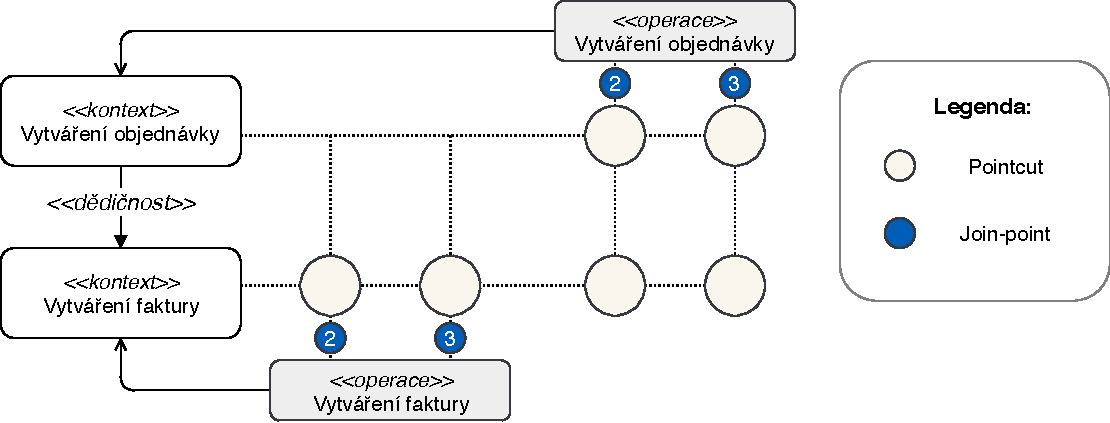
\includegraphics[keepaspectratio=true, width=1\linewidth]{figures/context-extension.pdf}
    \caption{Dědičnost kontextů ve vztahu k join-pointům a pointcuts}
    \label{fig:context-extension}
\end{figure}

\subsection{Advices}

V případě join-pointu~\ref{itm:initialization} je advice samotná reprezentace byznysového
kontextu přenášeného mezi službami. Naopak v join-pointech~\ref{itm:before}~a~\ref{itm:after}
je přidanou funkcionalitou vyhodnocování preconditions nad aplikačním kontextem, resp. aplikování
post-conditions na návratovou hodnotu operace.

\subsection{Weaving}

Weaving v případě join-pointu~\ref{itm:initialization} bude provádět komponenta frameworku, která
analyzuje lokálně dostupná pravidla služby, vyhodnotí, která pravidla je potřeba stáhnout,
a vyžádá tato pravidla od příslušných služeb.
V případě join-pointů~\ref{itm:before}~a~\ref{itm:after} je k weavingu potřeba využít speciální aspect
weaver. Ten zachytí volání byznysové operace a získá informace o aktuálním stavu aplikačního kontextu.
Následně zjistí, který byznysový kontext má být aplikován, shromaždí všechny preconditions
a každou z nich vyhodnotí. Pokud některá precondition není splněna, byznysová operace je zastavena
a je vyhozena výjimka, kterou služba zpracuje. V opačném případě je kontrola vrácena zpět
službě, která vykoná byznysovou operaci. Po dokončení operace aspect weaver zachytí výstup byznysové
operace a aplikuje post-conditions daného byznysového kontextu. Proces weavingu je zachycen na
obrázku~\ref{fig:business-rules-weaver}.

\begin{figure}
    \centering
    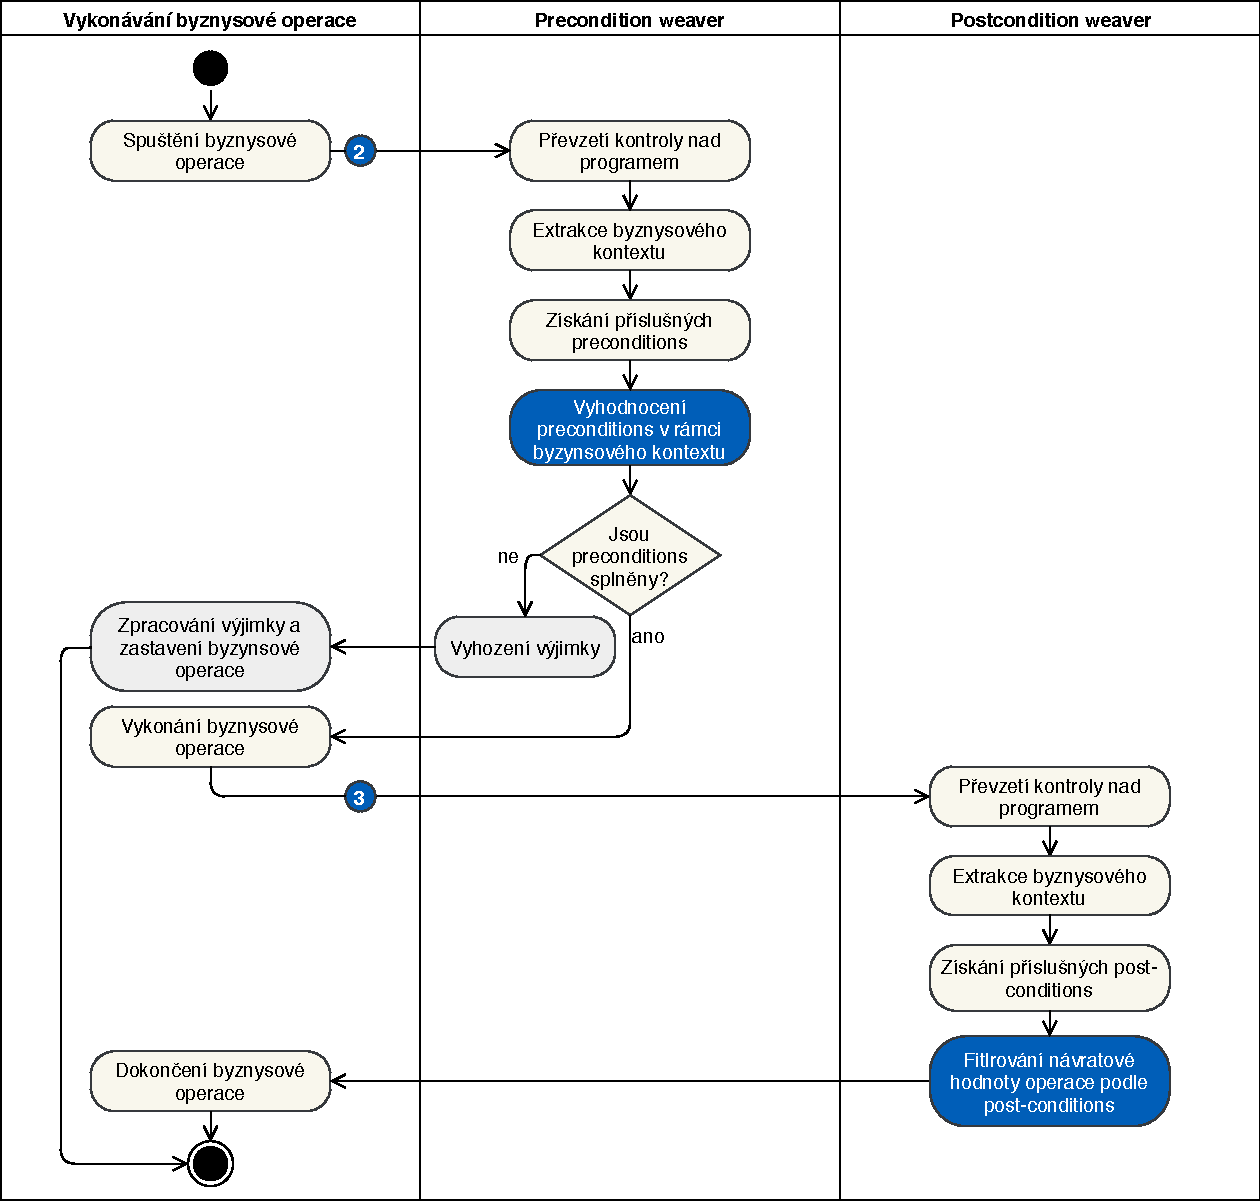
\includegraphics[keepaspectratio=true, width=0.8\linewidth]{figures/business-rules-weaver.pdf}
    \caption{Proces weavingu byznysov\'ych pravidel}
    \label{fig:business-rules-weaver}
\end{figure}

\section{Dědičnost byznysových kontextů}\label{sec:context-inheritance}

V předchozím textu byl představen koncept dědičnosti byznysových kontextů.
Každý kontext díky němu může rozšiřovat libovolné množství jiných kontextů, a sdílet jejich
byznysová pravidla. Byznysové operace pak mohou samy určit, který byznysový kontext se k ním váže.
Tento kontext však přináší několik problémů, které jsou rozebrány v následujících odstavcích.

Může nastat situace, kdy je potřeba sdílet pouze některá byznysová pravidla
daného kontextu. Při mapování kontextů jedna ku jedné s operacemi by to ale
nebylo možné. Řešením je využití tzv. \textit{abstraktních kontextů},
které přímo nevyužívá žádná byznysová operace.
Příklad znázorněný na obrázku~\ref{fig:abstract-context} popisuje situaci, kdy je nežádoucí,
aby kontext \code{user.register} zdědil pravidlo vyžadující přihlášení uživatele.

\begin{figure}
    \centering
    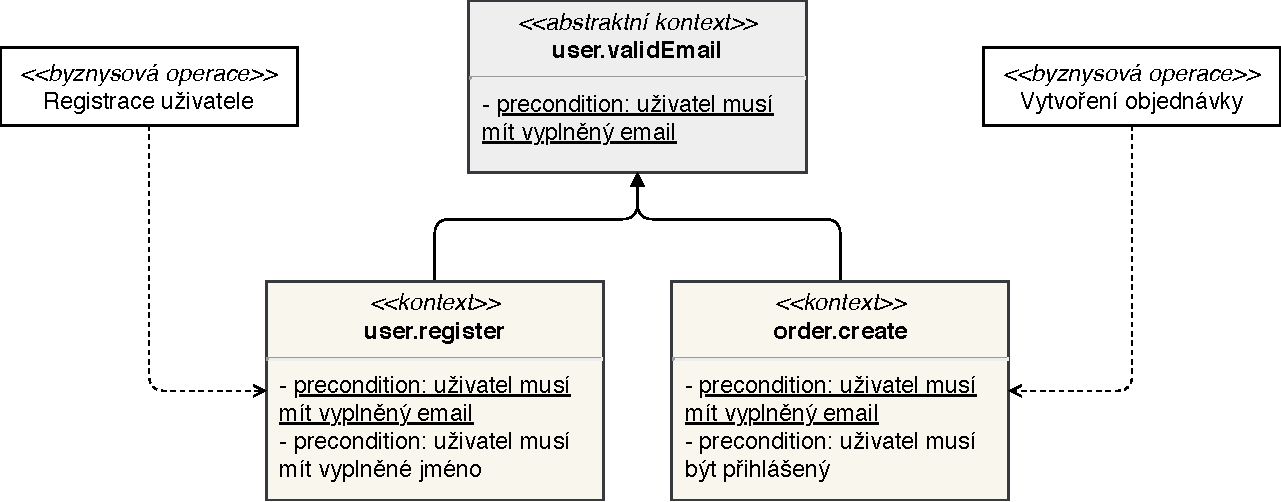
\includegraphics[keepaspectratio=true, width=1\linewidth]{figures/abstract-context.pdf}
    \caption{Znázornění abstraktního byznysového kontextu}
    \label{fig:abstract-context}
\end{figure}

Kvůli dědičnosti může vzniknout v grafu závislostí kontextů cyklus, který by způsobil zacyklení
procesu inicializace v~\ref{itm:initialization}. Tuto situaci nelze z hlediska frameworku vyřešit,
ale dá se jí předejít. K prevenci by mohl sloužit validátor vestavěný do nástroje pro správu
byznysových kontextů.

Vícenásobná dědičnosti může přinést problém, kdy jeden kontext zdědí více stejných pravidel z
různých zdrojů, tzv. \textit{diamond problem}~\cite{boyen1994generalized}. Tomu lze předejít tak, že
každé pravidlo bude mít unikátní identifikátor v rámci celého systému a při dědění budou zohledněna
pouze unikátní pravidla. Zajištění unikátního identifikátoru lze zajistit díky nástroji pro centrální
administraci byznysových pravidel.

\section{Logické výrazy byznysových pravidel}

Sekce~\ref{sec:business-rules} uvádí, že pravidla obsahují logické podmínky. V případě preconditions je to
ověření podmínky, která musí být platná před spuštěním byznysové operace v~\ref{itm:before}. V případě
post-condition může filtrování návratové hodnotry podléhat splnění určité podmínky, která musí být
vyhodnocena v~\ref{itm:after}.

\begin{figure}
    \centering
    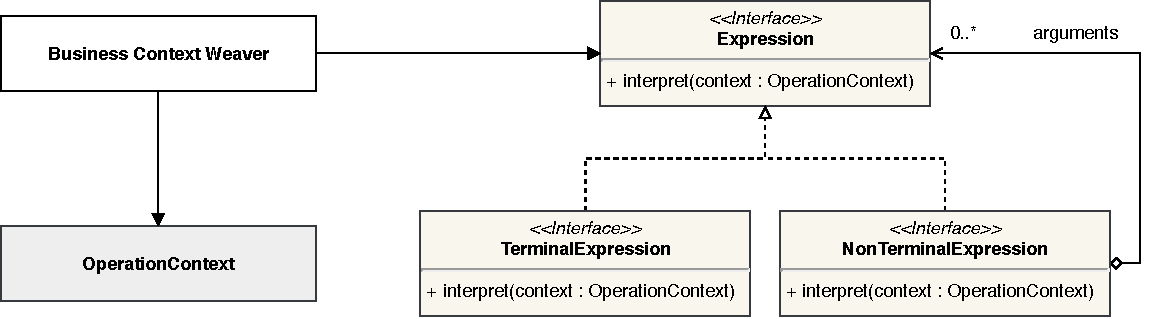
\includegraphics[keepaspectratio=true, width=1\linewidth]{figures/expression.pdf}
    \caption{Použití vzoru Intepreter pro vyhodnocování logických výrazů}
    \label{fig:expression}
\end{figure}

Podmínky byznysových pravidel se skládají z jednotlivých výrazů, které tvoří
orientovaný acyklický graf (\gls{DAG}), tzv. \textit{derivační strom}.
Výrazy se dělí na \textit{terminály} a \textit{neterminály}~\cite{melichar2003jazyky}.
Terminál znamená, že z daného výrazu již nevychází žádná hrana do jiného výrazu.
Neterminál je opak terminálu. Pro reprezentaci stromu bude využit návrhový vzor
\textit{Composite}~\cite{fowler2002patterns}. K vyhodnocování podmínek popsaných v byznysovém
pravidle je vhodný návrhový vzor \textit{Interpreter}~\cite{fowler2002patterns}, jehož
použití je demonstrováno na obrázku~\ref{fig:expression}.

Framework bude disponovat základní sadou výrazů pro zápis byznysových pravidel.
Mezi ně budou patřit logické operace \code{and}, \code{or}, \code{equals} a \code{negate}.
Dále výraz \code{VariableReference}, který získá hodnotu proměnné či konstanty z kontextu.
Pokud bude v kontextu uložen objekt, je potřeba přistupovat i k jeho
veřejným atributům, což bude zajišťovat výraz \code{ObjectPropertyReference}.
K ověření přítomnosti hodnoty v proměnné bude sloužit výraz \code{IsNotNull}. Výraz \code{IsNotBlank} ověří,
zda je v proměnné řetězec nenulové délky. Pro vložení konstantní hodnoty přímo do byznysového pravidla bude
sloužit terminál \code{Constant}. Pro zvýšený komfort budou přidány i výrazi realizující základní matematické operace sčítání, odečítání,
násobení a dělení. Pro volání uživatelských funkcí definovaných v operačním kontextu bude sloužit speciální výraz
\code{FunctionCall}. V jeho případě je nutno zohlednit skutečnost, že funkce může přijímat libovolný počet argumentů.
Protože volaná funkce může potřebovat přistupovat k operačnímu kontextu, musejí být argumenty také interpretovány.
Bohužel nelze u uživatelem definovaných funkcí ověřit, že bude při jejich volání odpovídat počet a typ argumentů.
Přehled všech výrazů, které bude framework podporovat, je v tabulce~\ref{tbl:expressions},

\afterpage{%
\clearpage% Flush earlier floats (otherwise order might not be correct)
\begin{landscape}
    \begin{table}
        \centering
        \begin{tabular}{ l l l c c }
            \hline
            \textbf{Název} & \textbf{Argumenty} & \textbf{Atributy} & \textbf{Návratový typ} & \textbf{Typ výrazu} \\ \hline \hline
            \textbf{Constant} & - & Hodnota a typ konstanty & \code{?} & Terminál \\
            \textbf{FunctionCall} & Libovolný počet argumentů & Návratový typ funkce & \code{?} & Terminál \\
            \textbf{IsNotNull} & Jeden argument libovolného typu & - & \code{BOOL} & Neterminál \\
            \textbf{IsNotBlank} & Jeden argument typu \code{STRING} & - & \code{BOOL} & Neterminál \\
            \textbf{LogicalAnd} & 2 argumenty typu \code{BOOL} & - & \code{BOOL} & Neterminál \\
            \textbf{LogicalEquals} & 2 argumenty libovolného typu & - & \code{BOOL} & Neterminál \\
            \textbf{LogicalNegate} & 1 argument typu \code{BOOL} & - & \code{BOOL} & Neterminál \\
            \textbf{LogicalOr} & 2 argumenty typu \code{BOOL} & - & \code{BOOL} & Neterminál \\
            \textbf{NumericAdd} & 2 argumenty typu \code{NUMBER} & - & \code{NUMBER} & Neterminál \\
            \textbf{NumericSubtract} & 2 argumenty typu \code{NUMBER} & - & \code{NUMBER} & Neterminál \\
            \textbf{NumericMultiply} & 2 argumenty typu \code{NUMBER} & - & \code{NUMBER} & Neterminál \\
            \textbf{NumericDivide} & 2 argumenty typu \code{NUMBER} & - & \code{NUMBER} & Neterminál \\
            \textbf{ObjectReference} & - & Název objektu a název a typ proměnné & \code{?} & Terminál \\
            \textbf{VariableReference} & - & Název a typ proměnné & \code{?} & Terminál \\
            \hline
        \end{tabular}
        \caption{Přehled výrazů pro zápis byznysového pravidla}
        \label{tbl:expressions}
    \end{table}
\end{landscape}
\clearpage% Flush page
}

%\goal{Typované výrazy}
Pro snažší implementaci na více platformách a prevenci sémantických chyb v pravidlech budou výrazy
obsahovat i explicitní definici svého návratového typu. Výraz byznysového pravidla může nabývat logických hodnot,
může vracet číslo, textový řetězec a také objekt. Je potřeba počítat také s tím, že výraz nevrací žádnou
hodnotu.

\begin{itemize}
    \item \code{BOOL} je logický typ, který nabývá hodnoty \code{true} a \code{false}.
    \item \code{NUMBER} je reálné číslo zapsáno ve tvaru s desetinnou tečkou a neomezeným počtem číslic.
    \item \code{OBJECT} je objekt libovolného typu.
    \item \code{STRING} je textový řetězec.
    \item \code{VOID} je pseudotyp značící, že výraz nemá návratovou hodnotu.
\end{itemize}

%\goal{Atributy pravidel}
Kromě argumentů neterminálů je v některých případech potřeba k výrazu uložit i dodatečné informace \textendash\xspace
\textit{atributy}. Jedním z atributů je typ návratové hotnoty výrazu, pokud není přímo implikována.
V případě výrazu \code{Constant} je potřeba uložit hodnotu a typ konstanty. Reference na proměnnou
musí obsahovat její název a typ, reference na pole objektu navíc musí obsahovat název odkazovaného pole.
Volání funkce musí obsahovat její název a návratový typ.

\begin{figure}
    \centering
    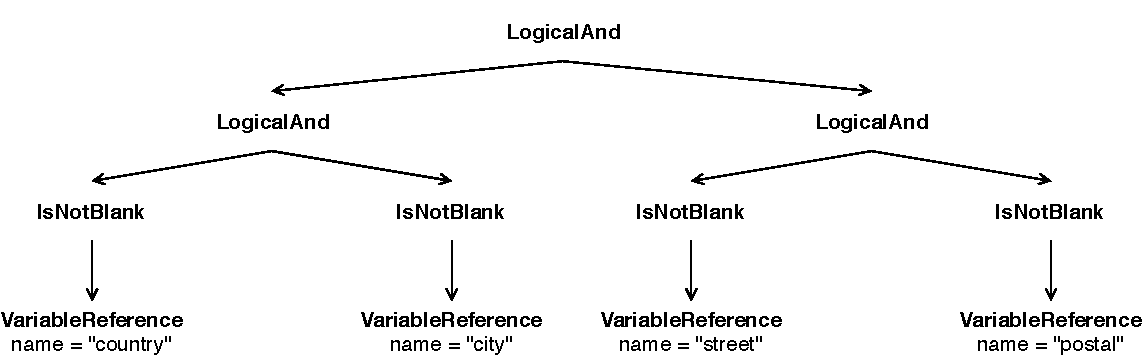
\includegraphics[keepaspectratio=true, width=1\linewidth]{figures/simple-rule.pdf}
    \caption{Syntaktický strom jednoduchého validačního pravidla}
    \label{fig:simple-rule}
\end{figure}

%\goal{Příklad AST pravidla}
Na obrázku~\ref{fig:simple-rule} je znázorněn syntaktický strom, který zachycuje jednoduché
validační pravidlo validující fakturační adresu. Jedná se o ekvivalent validačních pravidel
zachycených ve zdrojovém kódu~\ref{lst:jsr303} pomocí anotací standardu \gls{JSR} 303.
Pravidlo je tvořeno čtyřmi teminály, které se odkazují na proměnné operačního kontextu.
Hodnoty proměnných jsou validovány výrazem \code{IsNotBlank} a jednotlivé validace
jsou spojeny pomocí binárních výrazu \code{LogicalAnd} odpovídajících logické konjunkci.

\section{Filtrování návratových hodnot byznysové operace}

Při aplikování post-conditions je filtrována návratová hodnota byznysové operace. Tou může být proměnná
obsahující číslo, text, objekt, či jejich kolekce. Filtrování jednoduchých hodnot nemá pro byznysová pravidla reálný přínos.
V případě objektu lze filtrovat jeho atributy, například skrýt e-mailovou adresu uživatele.
V případě kolekce lze filtrovat jejich prvky, například skrýt objednávky, které uživateli nepatří.
Pokud se v kolekci nachází objekty, lze požadovat, aby byly zakryty atributy jednotlivých objektů,
například filtrování e-mailových adres v kolekci více uživatelů. Itentifikovanými typy post-conditions tedy jsou:

\begin{itemize}
    \item \code{FILTER\_OBJECT\_FIELD} filtruje atribut objektu, který je výstupem operace.
    \item \code{FILTER\_LIST\_OF\_OBJECTS} filtruje objekty v kolekci, která je výstupem operace.
    \item \code{FILTER\_LIST\_OF\_OBJECTS\_FIELDS} filtruje atributy objektů v kolekci, která je výstupem operace.
\end{itemize}

\section{Metamodel byznysového kontextu}\label{sec:metamodel}

\begin{figure}
    \centering
    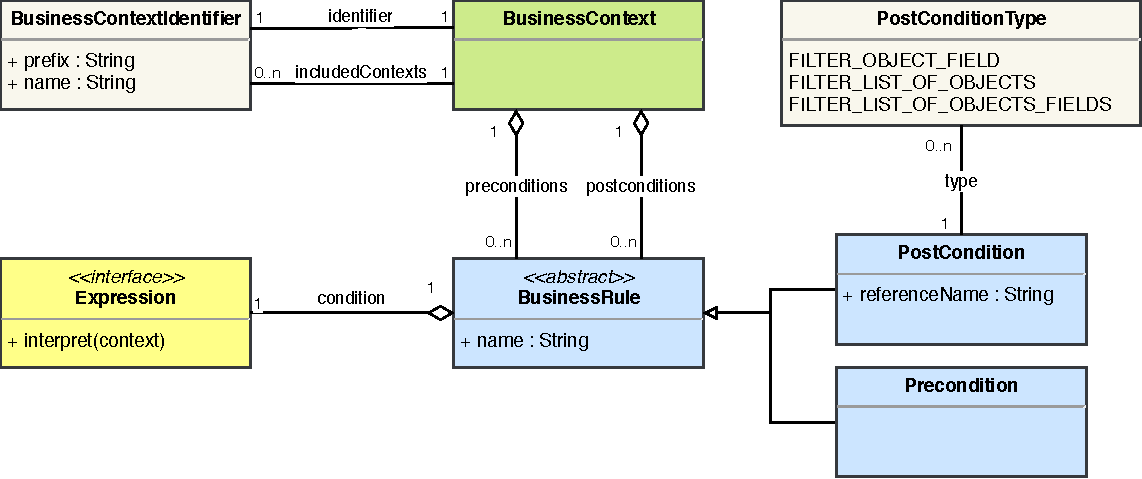
\includegraphics[keepaspectratio=true, width=\linewidth]{figures/business-context-metamodel.pdf}
    \caption{Metamodel byznysového kontextu}
    \label{fig:business-context-metamodel}
\end{figure}

Z předchozího textu vyplývá podoba metamodelu byznysových pravidel, resp. byznysových kontextů.
Kromě samotných logických výrazů musí pravidlo nést informace o tom, zda
se jedná o precondition nebo post-condition, a také jeho identifikátor.
Post-condition navíc potřebuje uložit informaci o jejím typu a názvu. Pravidla jsou uskupována
do byznysových kontextů, z nichž každý má svůj unikátní identifikátor skládající se z prefixu
a samotného jména a seznam rozšířených kontextů. Diagram tříd navrženého kontextu je znázorněn
na obrázku~\ref{fig:business-context-metamodel}.

\section{Popis byznysových kontextů pomocí \gls{DSL}}

Př\'{\i}stup \gls{ADDA} doporučuje popsat byznysová pravidla pomoc\'{\i}
vlastn\'{\i}ho, na m\'{\i}ru šitého, doménově specifického jazyka~\cite{cemus2015automated}.
Pro účely frameworku bude popsán pomocí \gls{DSL} celý byznysový kontext.
Jak bylo popsáno v sekci~\ref{sec:business-rule-dsl}, vlastnosti nástrojů Drools a JetBrains MPS,
nejsou optimální pro dosažení vytyčených cílů. Pro účely frameworku je tedy nutné specifikovat vlastnosti,
které by \gls{DSL} mělo nést. Konkrétní podoba DSL bude přenechána na implementaci frameworku.

Pro uložení kontextu z metamodelu do \gls{DSL}, aby ho mohl vývojář či administrátor
systému upravovat, je vzhledem k reprezentaci logických výrazů vhodný návrhový vzor
\textit{Visitor}~\cite{fowler2002patterns}. Ten umožní převádět libovolně složité logické
výrazy pomocí metody \textit{double-dispatch}. Jeho volbou je zároveň zajištěna rozšiřitelnost
frameworku pro libovolné \gls{DSL} \textendash\xspace bude stačit implementovat konkrétní
visitor pro zvolený jazyk, aniž by bylo nutno zasahovat přímo do implementace frameworku.
Princip použití vzoru Visitor je znázorněn na obrázku~\ref{fig:expression-visitor}.

\begin{figure}
    \centering
    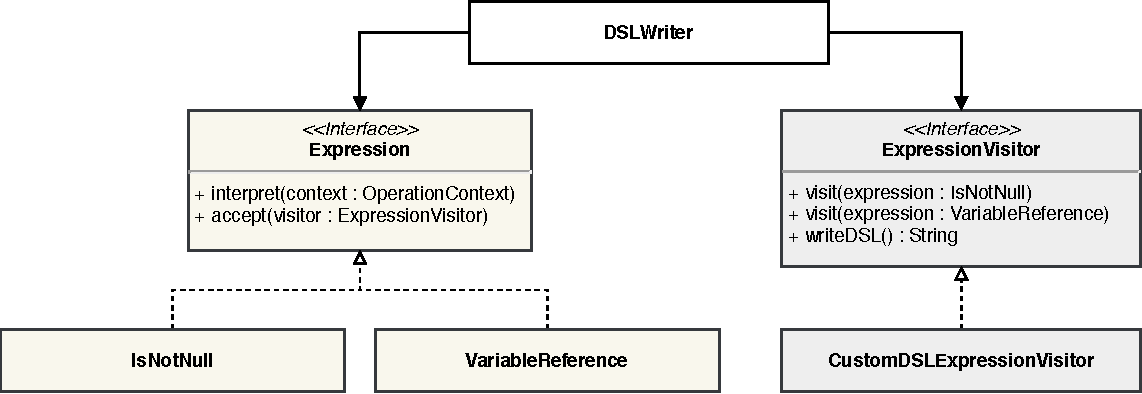
\includegraphics[keepaspectratio=true, width=1\linewidth]{figures/expression-visitor.pdf}
    \caption{Využití vzoru Visitor pro zápis logických výrazů v \gls{DSL}}
    \label{fig:expression-visitor}
\end{figure}

\section{Organizace byznysových kontextů}

Každá služba bude mít lokálně uložen popis byznysových kontextů, které se sémanticky vztahují
k její doméně. Pro snažší přidělení byznysových kontextů ke službám bude v identifikátoru kontextu sloužit
tzv. \textit{prefix}. Kontexty se stejným prefixem pak budou spravovány výhradně jednou službou. Například kontexty
služby spravující objednávky budou označeny prefixem \code{order}, zatímco kontexty služby zajišťující fakturaci budou
označeny prefixem \code{billing}. Může nastat i situace, kdy jedna služba bude spravovat více prefixů.

\subsection{Registr byznysových kontextů}

Cílem frameworku je soustředit byznysové kontexty na jedno místo, ze kterého budou
automaticky distribuovány. Pro tento účel bude využit registr byzynsových pravidel
(\code{BusinessContextRegistry}), který bude mít za úkol kontexty načítat z \gls{DSL} do metamodelu,
stahovat lokálně nedostupné kontexty z ostatních služeb a načtené kontexty uchovávat pro použití při weavingu.
Každá služba pak bude disponovat svým registrem. Při inicializaci kontextů spolu budou registry komunikovat
a vyměňovat si sdílené kontexty.

\subsection{Uložení kontextů}

Byznysové kontexty popsané pomocí \gls{DSL} mohou být v příslušné službě uloženy v souborech na disku či v
databázi. Navrhovaný framework by na způsobu uložení neměl být závislý a o potřebné kroky
pro načtení či případně uložení kontextu se postará konkrétní implementace. Pro tento účel
je tedy vhodné, aby registr pracoval s nekonkrétními rozhraními, na jejichž implementaci
nebude nijak záviset.

\section{Inicializace byznysových kontextů}

\begin{figure}
    \centering
    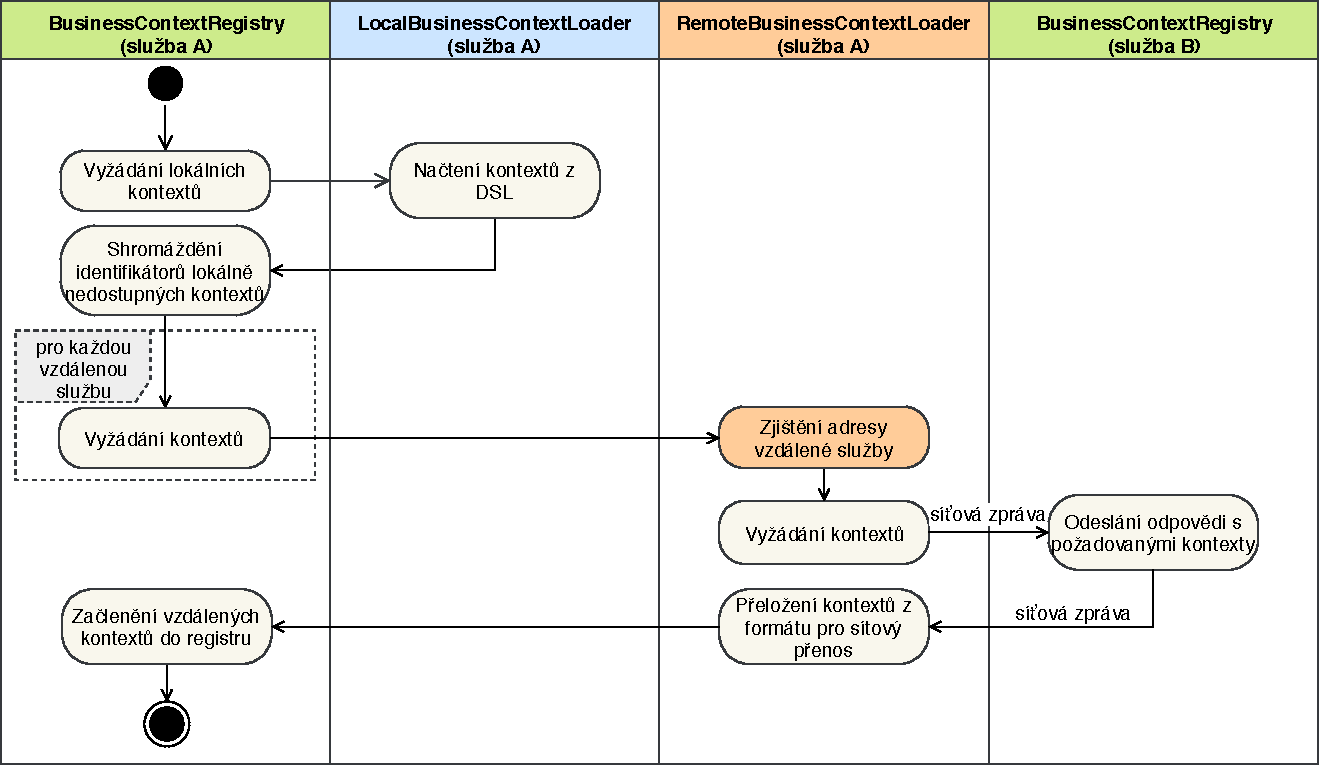
\includegraphics[keepaspectratio=true, width=\linewidth]{figures/business-context-loading.pdf}
    \caption{Proces inicializace byznysov\'ych kontextů}
    \label{fig:business-context-loading}
\end{figure}

Při inicializiaci byzynsových kontextů jsou nejprve načteny lokálně dostupné kontexty popsané pomocí \gls{DSL}.
Po převedení kontextů z \gls{DSL} do metamodelu je shromážděn seznam rozšířených kontextů a z nich jsou vybrány ty,
které nejsou lokálně dostupné. Následně jsou tyto vzdálené kontexty vyžádány od příslušných služeb
a po obdržení jsou převedeny ze síťového formátu do metamodelu. Nakonec jsou sdílená pravidla rozšířených kontextů začleněna
do kontextů, které od nich dědí. Celou inicializaci bude zastřešovat komponenta \code{BusinessContextRegistry}, která
má znalost o všech subsystémech, které jsou k tomuto procesu potřeba. Tato komponenta implementuje
návrhový vzor \textit{Facade}~\cite{fowler2002patterns}. Na obrázku~\ref{fig:business-context-loading} je znázorněn
navržený proces inicializace.

\section{Centráln\'{\i} správa byznysových kontextů}

Vzhledem k nutnosti centralizovat správu byznysových kontextů se
architektura \gls{P2P} představená v sekci~\ref{sec:p2p} nehodí.
Při úpravě kotextů by totiž v systému mohly existovat najednou staré i nové verze
byznysových pravidel, což je pro správnou funkci systému nepřijatelné.
Framework tedy využije architektury klient-server s více servery.
Byznysové kontexty budou podle prefixu přideleny službám, které budou
spravovat jejich aktuální a jediný stav a poskytovat je jiným službám.

\subsection{Uložen\'{\i} rozšířeného pravidla}\label{sec:saving-context}

Při ukládání byznysového kontextu je potřeba změnu propagovat do všech ostatních kontextů, které od něj dědí.
Při změně rozšířeného kontextu budou všechny služby, které ho využívají, informovány pomocí nástroje pro
centrální správu byzynsových pravidel. Ten má informaci o všech závislostech v systému a zároveň zná i adresu všech
služeb. Nevýhodou tohoto přístupu je zvýšená komunikační zátěž kvůli většímu objemu přenesených informací, stejný kontext
je totiž potřeba rozeslat mezi více služeb. Při implementaci je nutno zvážit, zda je tato zátěž vůči absolutnímu objemu
přenášených dat v systému významná. Bylo by vhodné vybrat vhodný přenosový formát, který minimalizuje dopad veškeré síťové
komunikace týkající se distribuce byznysových pravidel.

\subsection{Proces úpravy kontextu}

\begin{figure}
    \centering
    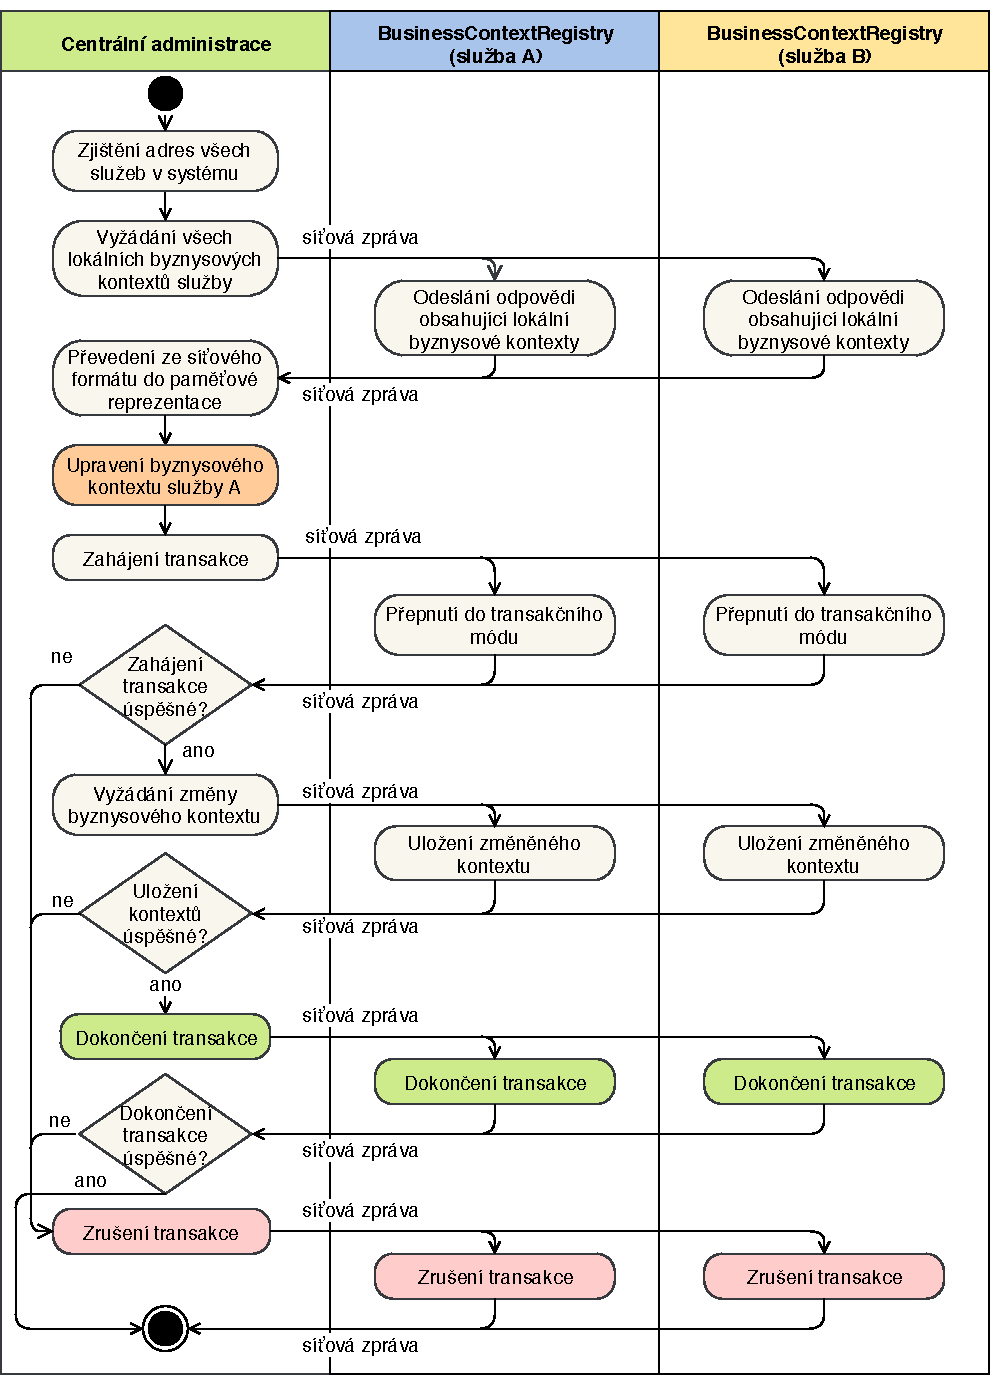
\includegraphics[keepaspectratio=true, width=\linewidth]{figures/business-context-management.pdf}
    \caption{Proces centráln\'{\i} správy byznysov\'ych kontextů}
    \label{fig:business-context-management}
\end{figure}

Proces úpravy byznysového kontextu pomocí nástroje pro centrální administraci nejprve načte všechny
byznysové kontexty všech služeb v systému. Následně zobrazí administrátorovi formulář pro úpravu pravidla.
Pravidlo je pro účely formuláře převedeno z metamodelu do \gls{DSL}. Po odeslání formuláře bude pravidlo
převedeno zpět do metamodelu. Nástroj pro administraci poté analyzuje, na které služby bude
mít změna pravidla dopad. Následně je s těmito službami zahájena transakce, při které v nich
nesmí probíhat žádná byznysová operace. Když všechny ovlivněné služby zahájí transakci, je možno
jim rozeslat novou podobu pravidla. Pokud vše proběhne v pořádku, je možno transakci dokončit
a služby otevřít byznysovým transakcím. Pokud naopak některý z kroků transakce selže, je nutno
informovat všechny zúčastněné služby o zrušení transakce a změnu inkriminovaného pravidla zrušit.
Na obrázku~\ref{fig:business-context-management} je celý proces znázorněn. Proces pro uložení
nového kontextu je analogický.

\section{Architektura frameworku}\label{sec:architecture}

V této sekci je popsána obecná architektura navrženého frameworku v rámci služby využívající
klasickou třívrstvou architekturu~\cite{fowler2002patterns}, která se skládá z prezentační,
aplikační a datové vrstvy. Každá z těchto vrstev může framework využívat
\textendash\xspace prezentační vrstva při validování vstupních polí formuláře, aplikační vrstva při
aplikaci byzynsových pravidel v byznysových operacích a datová vrstva při aplikaci post-conditions pro
filtrování dat při jejich získávání z databáze.

\begin{figure}
    \centering
    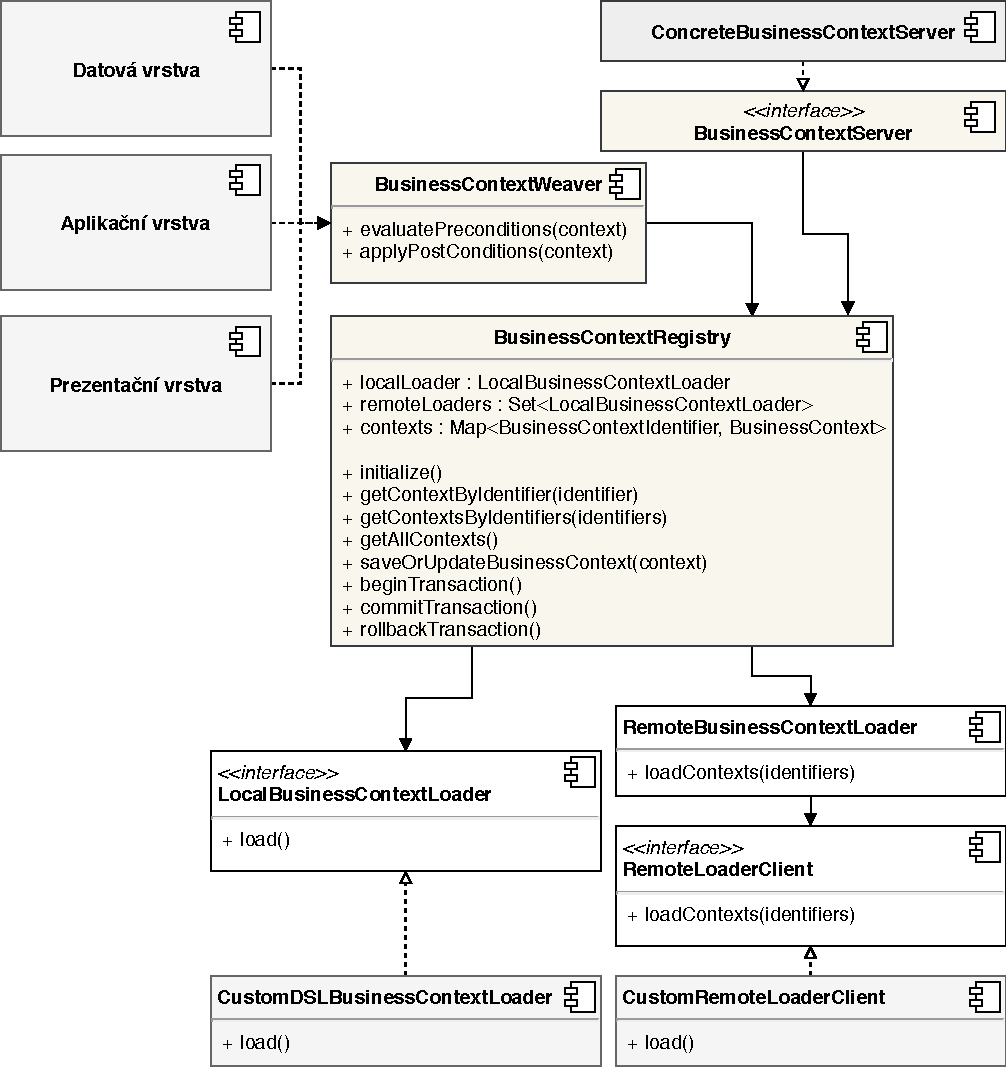
\includegraphics[keepaspectratio=true, width=\linewidth]{figures/business-context-registry.pdf}
    \caption{Architektura navrženého frameworku}
    \label{fig:business-context-registry}
\end{figure}

Základem frameworku je komponenta \code{BusinessContextRegistry}, tedy registr
byznysových kontextů, který je zodpovědný za inicializaci a uchovávání byznysových kontextů.
Načítání kontextů lze rozdělit na lokální a vzdálené. Při načítání lokálně dostupných kontextů
je potřeba získat \gls{DSL} kontextu ze souboru či databáze a převést ho do metamodelu.
K tomu bude využito rozhraní \code{LocalBusinessContextLoader}. Implementace rozhraní může být libovolná
a záviset na použitém \gls{DSL} či místu uložení pravidel. Naopak při načítání vzdálených
kontextů je potřeba vyžádat kontexty od vzdálené služby. O to se postará třída \code{RemoteBusinessContextLoader},
která požadované kontexty zorganizuje podle prefixu a poté pomocí rozhraní \code{RemoteLoaderClient} načte
pravidla od jednotlivých služeb. Implementace rozhraní \code{RemoteLoaderClient} bude záviset na použité
technologii a zajistí síťovou komunikaci a převod do a z formátu pro síťový přenos.
Aby mohl framework poskytovat lokální byznysové kontexty dané služby ke stažení, musí zastřešit
i serverovou funkcionalitu. K tomu slouží rozhraní \code{BusinessContextServer}. To bude využívat
\code{BusinessContextRegistry}, ze kterého načte byznysové kontexty, které si vyžádá \code{RemoteLoaderClient}.
Implementace serveru bude opět závislá na konkrétní technologii.
Nakonec bude framework obsahovat sadu aspect weaverů, které umožní weaving byznysových pravidel do
jednotlivých vrstev systému. Pro účely této práce bude framework poskytovat weavery pro využití v
aplikační vrstvě pro weaving preconditions a post-conditions do byznysových operací.
Architektura je zachycena na obrázku~\ref{fig:business-context-registry}.

\subsection{Service discovery}

% TODO: tohle možné nezmiňovat v samostatné kapitole, ale jen to zmínit při procesu načítání
Aby framework mohl distribuovat byznysové kontexty mezi službami, musí služba vyžadující kontext
znát adresu služby, od které ho vyžaduje. Adresy služeb mohou podléhat různým konfiguracím,
které se mohou lišit systém od systému. Framework proto nesmí být závislý na způsobu,
jakým se adresování služeb provádí. Nejlepším řešením je přenechat na uživateli frameworku, aby sám
získal a předal adresy služeb ve chvíli, kdy je framework potřebuje \textendash\xspace tedy
ve chvíli, kdy je potřeba načíst lokálně nedostupné kontexty.

\section{Shrnutí}

V této kapitole byl popsán návrh frameworku pro centrální správu a automatickou distribuci
byznysových pravidel v \gls{SOA} na základě přístupu \gls{ADDA}. Nejprve byla formalizována
doména byznysových pravidel v \gls{SOA} do názvosloví \gls{AOP}. Dále byla diskutována podobu byznysových pravidel,
jejich logických výrazů a jakým způsobem je lze zachytit v metamodelu a v \gls{DSL}.
Kapitola dále popisuje organizaci kontextů a procesy, kterými budou distribuovány a spravovány.
Nakonec byla shrnuta architektura frameworku.
